\documentclass[10pt,twocolumn]{article}
\usepackage[margin=0.75in]{geometry}
\usepackage[T1]{fontenc}
\usepackage{lmodern,amsmath,amssymb,booktabs,graphicx,hyperref,microtype}
\hypersetup{colorlinks=true,urlcolor=blue,linkcolor=blue}
\newcommand{\StructureCount}{3}
\newcommand{\EpisodeCount}{15}
\newcommand{\ProbeCount}{87}
\newcommand{\StateCount}{342,704}
\newcommand{\EdgeCount}{2,843,080}

\title{BrickPlan 1.2: Auditable Visual Diagnostics\\of Assembly-Order Errors and Recovery}
\author{Executable benchmark research release}
\date{October 5, 2026}
\begin{document}
\maketitle
\begin{abstract}
An assembly action can be physically admissible yet make later work more
expensive. BrickPlan measures this distinction using certified, finite
assembly transitions and exact completion costs. This revision corrects
trajectory-level measurement, replaces shortcut-prone continuation probes,
and adds matched raster-image and structured observation tracks.
The release contains \StructureCount{} structures from two source groups,
\EpisodeCount{} episodes and \ProbeCount{} probe responses.
All \StateCount{} reachable states and \EdgeCount{} directed transitions retain
the source geometry and fixed-path qualifications of the preceding release.
Thirty-six continuation pairs preserve initial observations, first and last
actions, and action multisets while changing interior order. A first--last
shortcut can no longer solve them. Self-induced feasibility losses now have
explicit detection, restoration and censoring records.
The revision also exposes a substantive limitation: a privileged static
relation rule solves all 15 episodes. Consequently, this is an auditable
diagnostic release, not evidence of search hardness or demonstrated VLM
shortsightedness. No model or human performance has been measured.
\end{abstract}

\section{Motivation and scope}
End-to-end assembly success conflates perception, immediate legality, future
access, and recovery. A closure can be installed correctly while blocking a
required interior insertion. Such an action is locally legal; rejecting it
using a goal-aware simulator would erase the error the benchmark seeks to
measure. BrickPlan therefore separates goal-independent execution from
evaluator-only future-feasibility labels.

Interactive reconstruction and assembly are established tasks, including
LTRON~\cite{ltron}, InstructioNet~\cite{instructionet},
LEGO-Puzzles~\cite{legopuzzles}, PhyBlock~\cite{phyblock}, and
Brick-Composer~\cite{composer}. Our contribution is the measurement and audit
contract linking legal decisions to later rework. We do not claim that
interaction, disassembly, or multi-step construction is new.

An adversarial audit of version 1.1 found that a static blocker-closure rule
solved every episode optimally and a first--last-action shortcut solved every
continuation probe. It also identified a hard-coded two-structure census in
the three-structure report, checkpoint-only dead-end measurement, and a
structured payload unsuitable for evaluating visual perception.
Version 1.2 repairs these concrete issues without overwriting frozen 1.0 or
1.1 artifacts. An increased episode length is not treated as increased
reasoning depth.

\section{Experimental design before empirical results}
\begin{table}[t]
\centering\small
\caption{Study conditions. These are unfilled experimental slots, not results.
Exact model identifiers, prompts, budgets and providers must be registered
before collection.}
\begin{tabular}{ll}\toprule
Condition & Status\\\midrule
Same VLM, image+ID, stepwise & Not evaluated\\
Same VLM, image+ID, explicit planning & Not evaluated\\
Same VLM, structured control & Not evaluated\\
Human, image+ID protocol & Not evaluated\\
Human, structured control & Not evaluated\\\bottomrule
\end{tabular}
\label{tab:study}
\end{table}
Each condition uses the same task starts, goals, identity seeds and action
budgets. Camera changes use the same inspection API for humans and agents.
The preregistration manifest records participant or model identity, provider
and version, prompt hash, temperature, reasoning setting, context and output
limits, provider cost cap, seed, track, timeout and retry policy.
The provider-neutral driver consumes public observations through an external
policy adapter. No provider calls are needed to reproduce the software controls.
Currency and model-token enforcement belong to that adapter; the executor
enforces action, inspection and diagnosis limits.

Evaluation runs have isolated stores and a fixed observation track.
Study mode permits one start per assigned episode and does not expose scores
or state replay. Administrative collection occurs on the evaluator host.
Policy processes must not have access to private banks, certificates, cost
tables, other tracks, or past study answers. Local practice is not this
isolation boundary.
Roadster and kart share one source kit and must remain in the same provenance
split. Repeated seeds are repeated runs, not additional structures.
Two provenance groups cannot support strong population-level inference.

\section{Certified workcell and tasks}
\subsection{Physical abstraction}
Each site is an original LDraw part instance at its original source pose.
A connected fixed subassembly is explicitly clamped. A mutable part may be
attached or detached along a specified straight translation if the path is
clear and the resulting assembly stays connected to the fixed base through
qualified stud connections. Connections are abstract rigid holds.
No artificial spacers, pose shifts, floating installed parts, or visually
substituted box meshes are introduced.

Version 1.2 reuses the geometry and path evidence frozen in 1.1. Closed
collision proxies are inset by 0.25 LDU per surface, with a 0.002 LDU guard.
Final-pose pairs must be clear; moving--obstacle pairs cover the full declared
translation. Interval clearance uses the 1-Lipschitz bound for surface
distance under translation; intersections witness obstruction. Unknown
geometry is inadmissible. These are numerical certificates within the
declared proxy/path domain, not physical experiments or free-motion guarantees.
The earlier source-verified repair of one missing 3022 proxy cap face remains
documented in the frozen provenance; display triangles are unchanged.

Let $s$ be mutable occupancy and $g$ the exact target occupancy. Local legality
uses only $s$, path blockers and connectivity, never $g$ or future costs.
Every legal transition has a verified inverse. Goal-rooted breadth-first search
provides $C^*(s,g)$, checked against the complete reachable component through
Bellman inequalities and decreasing-successor witnesses.
For $\Delta=|g|-|s|$, minimum detach count is
\[
D^*(s,g)=\frac{C^*(s,g)-\Delta}{2}.
\]
All task starts and completions have replayable witnesses. Hashes bind source,
geometry, transitions, tasks and cost tables; a trajectory also binds its full
task definition, including budgets.

\begin{table*}[t]
\centering\small
\caption{Certified bank and new partial-target reconfiguration episodes.
$C^*$ and $D^*$ refer to the reconfiguration start, not the full-build task.
Hamming distance counts initially mismatched sites.}
\begin{tabular}{llrrrrr}\toprule
Case & Source group & Sites & States & $C^*$ & $D^*$ & Hamming \\\midrule
roadster-body & LEGO-31027 & 17 & 14,012 & 30 & 14 & 4 \\
kart-deck & LEGO-31027 & 18 & 44,604 & 24 & 8 & 12 \\
airframe & LEGO-31028 & 21 & 284,088 & 34 & 15 & 8 \\
\bottomrule\end{tabular}

\label{tab:cases}
\end{table*}

\subsection{Episode protocols}
Each structure has five episodes: full build, safe continuation checkpoint,
injected repair, size-matched healthy control, and partial-target
reconfiguration. Full builds contain 17, 18 and 21 mutable pieces.
Injected repairs require exactly three detachments; their healthy controls
match installed count and inherit the repair budget.
Other action budgets are $C^*+\max(4,\lceil C^*/2\rceil)$.
Inspections have quota 32; diagnoses have quota 8.
Rejected structural attempts consume one action.

Reconfiguration starts contain both pieces absent from the final goal and
missing required pieces. A legal, goal-directed attachment exists that adds
two completion actions. Each start also has an optimal legal alternative.
These tasks exercise temporary access restoration over 24--34 actions, but
they retain the known access-order mechanism.
Exhaustive empty-to-state analysis found no temporary-scaffold construction
in any inherited bank. A deterministic search over existing goals and 30
additional reachable partial goals per structure found no example meeting
our stronger ``every legal required removal is worse than an available
installation'' criterion. This negative search is not an impossibility proof
over arbitrary source models, and support rerouting is not claimed.

\subsection{Matched continuation and counterfactual probes}
For each structure, 24 continuation probes form 12 pairs at lengths 4, 6 and
8. Every interior position from 2 through length minus 1 receives one
geometric conflict and one matched executable control. Both plans include
attachments and detachments; control steps are actual state changes.
We construct a legal walk and swap two interior actions, accepting it only
when authoritative replay first fails with motion obstruction or unsupported
assembly at the prescribed position. Duplicate-install and empty-removal
errors are excluded as the defining conflict.

The pair shares initial state, goal, randomized physical IDs, first action,
last action, length and action multiset. Only interior order differs.
Thus any classifier restricted to those invariant features gives the same
prediction for both members and has at most 50\% exact pair accuracy.
The actual first--last transition shortcut obtains 36/72 correct; full
transition replay obtains 72/72. This establishes resistance to that shortcut,
not immunity to all shortcuts or a bound on a model's internal search.

Three inherited one-step choice probes and 12 counterfactual member responses
complete the 87-response bank. Counterfactuals change the visible future
goal while keeping initial state and offered actions fixed. Each source has
one uniquely switching pair and one invariance pair. Evaluation uses exact
conditional cost $Q^*(s,a,g)=1+C^*(T(s,a),g)$ and normalizes independently
permuted candidate positions. These labels are defined among offered actions.

\section{Matched observation tracks}
The image+ID track exposes four PNG raster panels: current assembly with P/S
callouts, target with S callouts, all-site reference, and a catalog of site
shapes and available P inventory. Opaque P and S ID lists support action
selection; their permutations remain stable within a trial. Original LDraw
triangles are transformed and rasterized on the evaluator server using a
z-buffer. Only pixels leave the renderer. A visible-part callout requires
visible surface pixels; geometry, depth, object masks and connectivity are
not serialized into the policy payload.

The structured control receives the same images plus calibrated site
matrices, types, directions, occupancy and target flags. These fields are
explicitly privileged relative to image+ID, but still omit private blocker
relations and costs. The visual HTTP server has no mesh, geometry-file or
three.js scene-download route. It serves a canvas UI from the same raster
observations the API agent receives.

The initial isometric view is free. Each subsequent inspect request selects
one of seven fixed views or an exploded-reference diagram and consumes one
inspection. Exploding changes only the all-site reference; current and target
assemblies retain original poses. The same view changes apply to all panels.
There is no free orbit during scored interaction. Probe inspection budgets
persist across reloads, and answers are frozen once submitted.
These are known-pose placement diagnostics with visual input, not
unconstrained pose estimation or robot grasp planning.

\section{Seven measurement dimensions}
\paragraph{Dead-end choice rate.}
Define attach-only viability
$V^+(s,g)=[s\subseteq g\land C^*(s,g)=|g|-|s|]$, and no-rework viability
$V^0(s,g)=[C^*(s,g)=|s\triangle g|]$.
The latter allows necessary deletion of extra pieces but no temporary reversal
of an already matched site. Budget viability is
$V_B(s,g,b)=[C^*(s,g)\leq b]$.
For each predicate, an online legal decision is eligible only if the
predecessor is viable and both safe and unsafe legal alternatives exist.
The numerator counts chosen viability losses within that denominator.
Invalid actions are reported separately; they cannot enter a legal-choice
denominator, but may destroy budget viability.
One-step probe rates remain separate from online rates.

\paragraph{Lookahead depth.}
Score the exact first failing action, or null for a fully executable plan.
Report balanced accuracy and coverage both by plan length and by the
matched pair's actual conflict position. Conflict recall and valid-control
false alarms accompany accuracy; missing and invalid responses remain
visible. A supplied-plan distance curve is not a certified internal reasoning
depth, nor does a legal continuation necessarily reach the task goal.

\paragraph{Plan survival curve.}
Freeze the first attempted-action index losing each predicate.
Restoration does not erase a historical loss. Within each case, protocol,
optimal length and budget stratum, report known survivors, losses and
censored trials, with bounds $[A_t/N,(A_t+U_t)/N]$.
Missing episodes are censored even at time zero; a successful terminated
trial is absorbing. Default reports have one run per task, so curves are
descriptive records rather than reliable population estimates.

\paragraph{Regret.}
For successful episodes, action regret is attempted actions minus initial
$C^*$; detach regret is successful detach operations minus initial $D^*$.
Failed and unfinished episodes have null regret and explicit consumed costs.
Conservation gives
\[
R_{\mathrm{action}}=2R_{\mathrm{detach}}+N_{\mathrm{invalid}}.
\]
These are correlated views of cost, not independent evidence.
Legal-action Bellman excess is separately observable to the evaluator:
$1+C^*(s_{t+1},g)-C^*(s_t,g)$.

\paragraph{Recovery rate.}
A self-induced event begins when a legal action changes $V^0$ from true to
false. The first diagnosis after that event is retained, even when earlier
successful structural actions occurred. Its sign, attempt lag, and coverage
are explicit. An event restores when $V^0$ becomes true again; a new later
loss creates a new event. Terminal unrestored events differ from censored,
unfinished events. Report restoration and joint detection/restoration over
all events, plus an upper bound including censored outcomes.
Injected-repair detection and completion remain a separate protocol.
Absolute unreachability is not implied: the certified component is reversible.
Budget loss is separately irreversible because spent actions cannot be refunded.

\paragraph{Replanning efficiency.}
For every self-induced event, retain attempts and detachments through
restoration, exact cost and minimum detachments at entry, and prefix excess
$k+C^*(s_{\mathrm{restore}},g)-C^*(s_{\mathrm{entry}},g)$.
Report these costs alongside event coverage and restoration, not only for
successful survivors. Episode-level detach count, distinct removed P IDs and
failed attempts remain available. Diagnoses are also scored once per
distinct visited state, preventing repeated answers at one state from
inflating aggregate accuracy.

\paragraph{Counterfactual consistency.}
Joint correct switching requires correct offered choices in both changed-goal
members. Correct invariance requires correctness in both control members.
Switching alone is insufficient; a consistently wrong pair receives no joint
credit. Missing-member coverage and presented candidate positions are explicit.

\section{Software evidence and adversarial controls}
\begin{table}[t]
\centering\small
\caption{Software controls, not VLM or human scores. Runs reuse the same
15 tasks; denominators are task-runs, not independent structures.}
\begin{tabular}{lrr}\toprule
Software control & Runs & Success \\\midrule
oracle & 1 & 15/15 \\
static-relations & 1 & 15/15 \\
search-1 & 3 & 27/45 \\
search-2 & 3 & 27/45 \\
search-4 & 3 & 27/45 \\
public-greedy & 3 & 7/45 \\
legal-random & 3 & 0/45 \\
blind-random & 3 & 0/45 \\
\bottomrule\end{tabular}

\label{tab:controls}
\end{table}
The exact-oracle ceiling completes all 15 episodes with zero regret and scores
all probes correctly. A privileged static rule computes the transitive closure
of occupied blockers plus unwanted pieces, removes that set in legal order,
then greedily installs missing target parts without prematurely blocking
other missing parts. It also solves 15/15 episodes. This control selects no
actions using the cost tables and performs no state-space search.
The source graph remains private, so its success does not establish that the
visual task is solved; it does refute a claim that these episodes inherently
require deep search given perfect relations.

Depth-1, depth-2 and depth-4 bounded search use the private transition model,
Hamming leaf estimates and visited-state tie-breaking, without cost oracles.
All solve 9/15 tasks in each repeated run. This non-improvement is a
property of these controls, not a model capability result.
The public structured greedy policy uses only target flags, type
compatibility, observed IDs and rejection memory; its three seeds solve
2, 2 and 3 episodes. Uniform legal-action random has a privileged validity
set. Blind random samples public P/S IDs without reading pixels.
Neither random policy is forced to select known traps.
No control observes fabricated model outputs or hand-inserted wrong answers.

Semantic validation replays all 15 witnesses in both observation tracks,
checks all 36 matched pairs in private and public form, and exercises
self-induced diagnosis after successful actions, restoration, recurrence,
censoring, invalid attempts, report census, missing survival, and replay
tampering. HTTP checks cover both tracks, all probe kinds, revision and
idempotence, persisted view budgets, source-route rejection and study
restrictions. Six Firefox sessions complete injected repair and
reconfiguration for every structure through actual UI controls, including
inspection, diagnosis, replay, public export and feedback. These are
software acceptance trials using reference actions.

\begin{figure*}[t]
\centering
\begin{minipage}{.48\textwidth}\centering
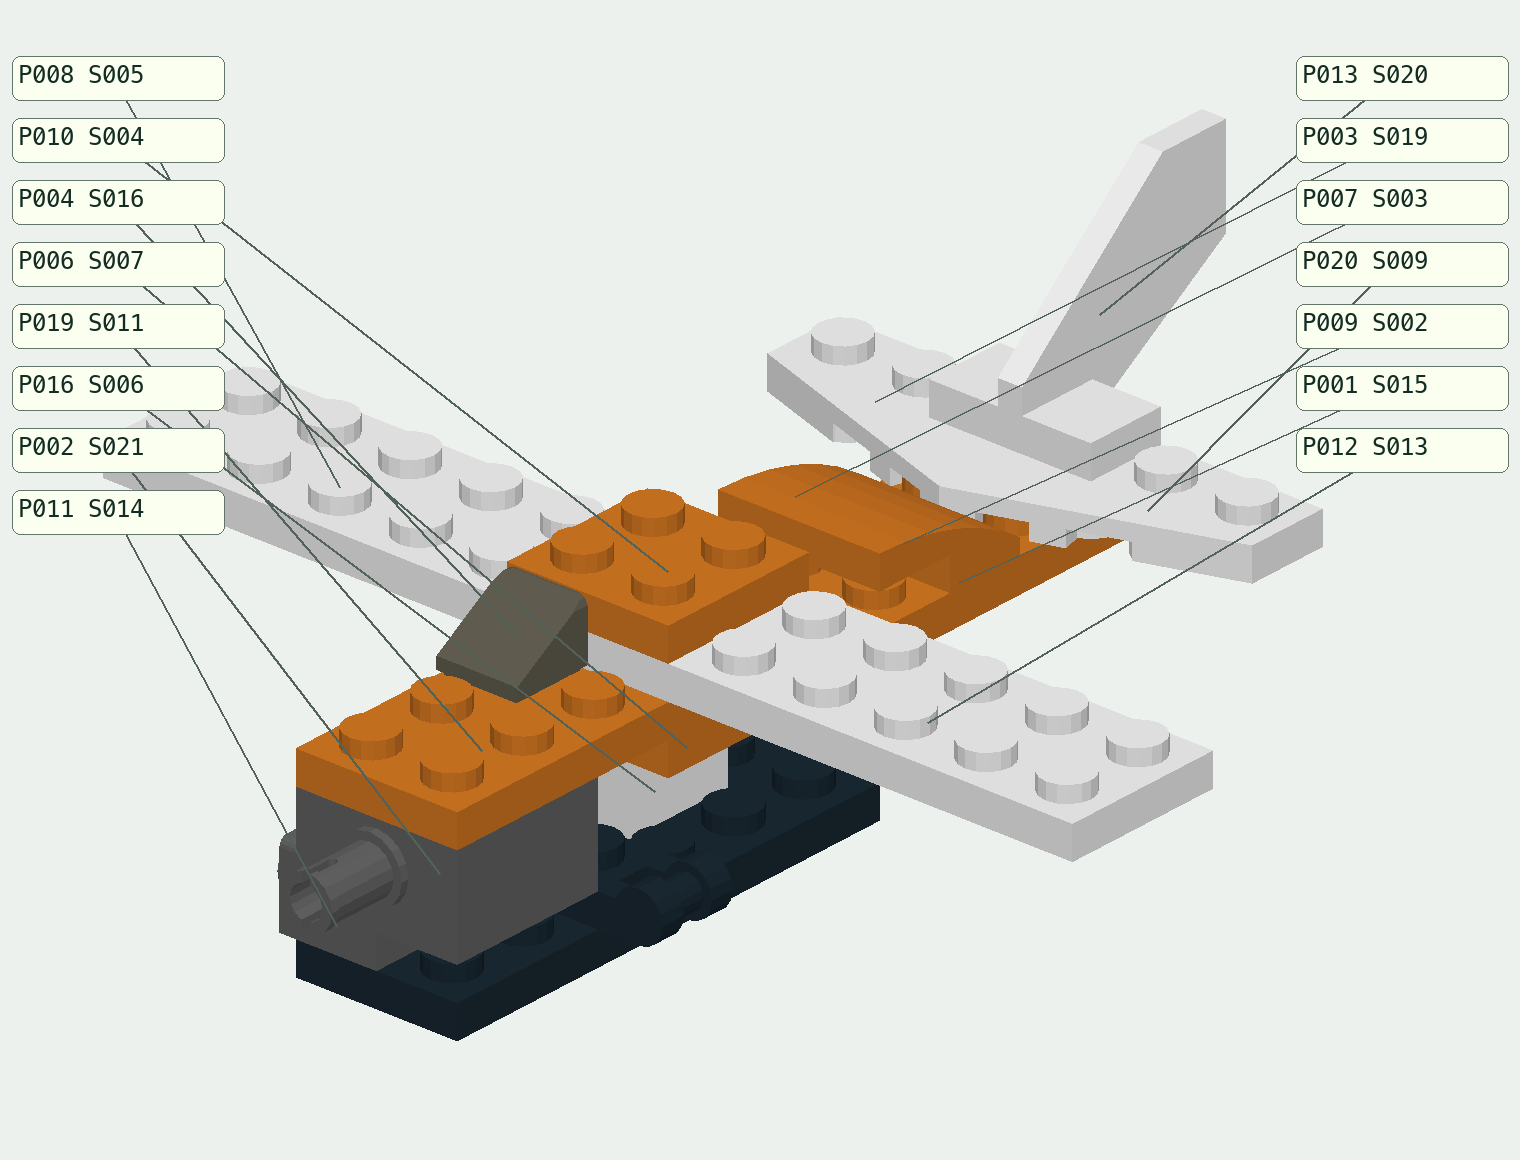
\includegraphics[width=\linewidth]{figures/reconfigure-0.png}\\
\small (a) Reconfiguration start, action 0.
\end{minipage}\hfill
\begin{minipage}{.48\textwidth}\centering
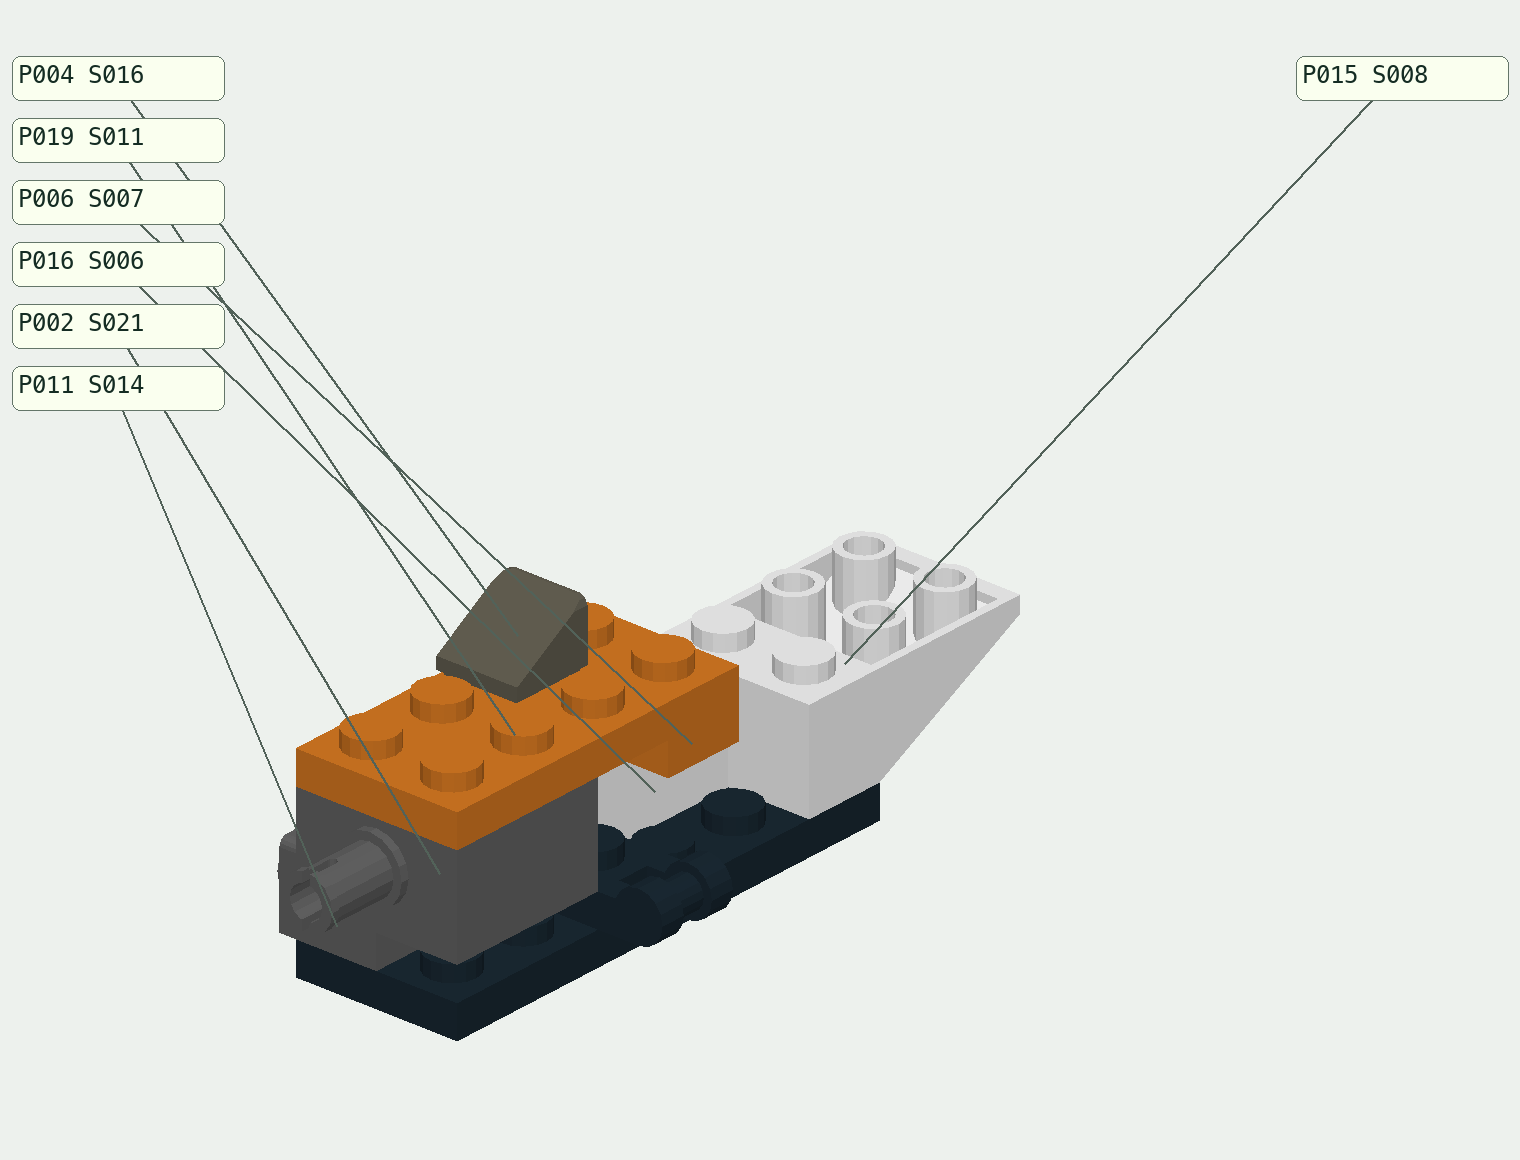
\includegraphics[width=\linewidth]{figures/reconfigure-10.png}\\
\small (b) After 10 successful actions.
\end{minipage}
\medskip

\begin{minipage}{.48\textwidth}\centering
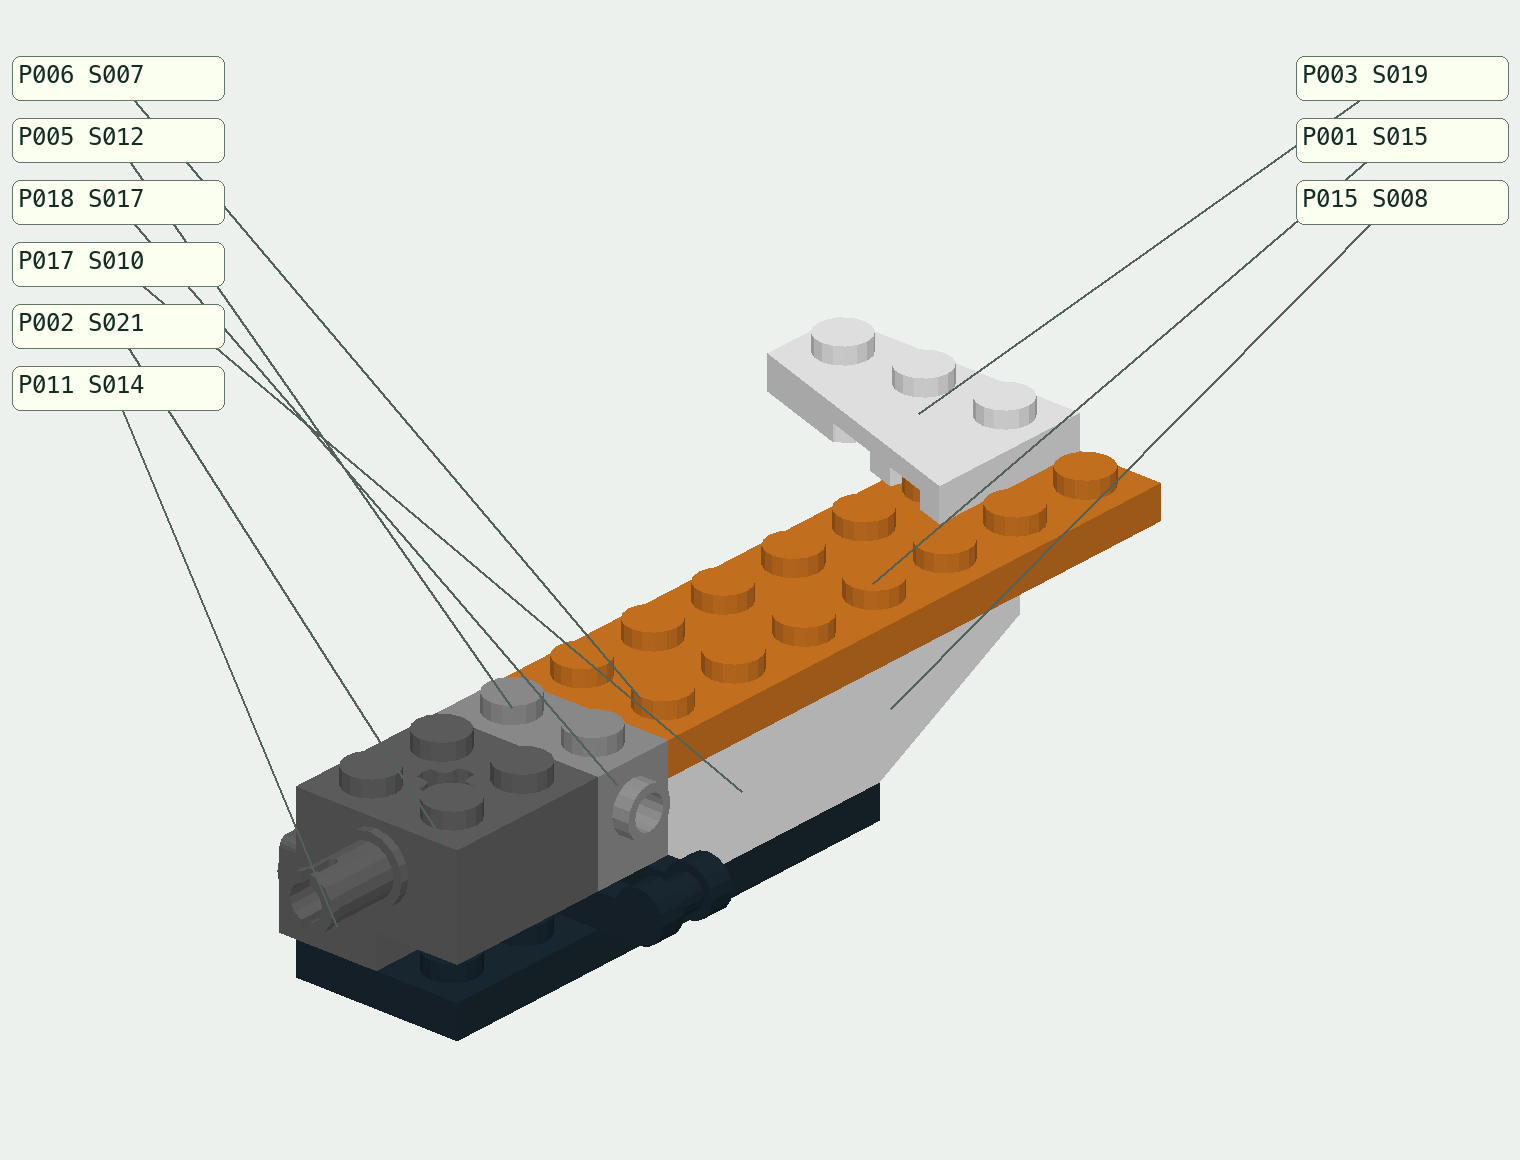
\includegraphics[width=\linewidth]{figures/reconfigure-20.png}\\
\small (c) After 20 successful actions.
\end{minipage}\hfill
\begin{minipage}{.48\textwidth}\centering
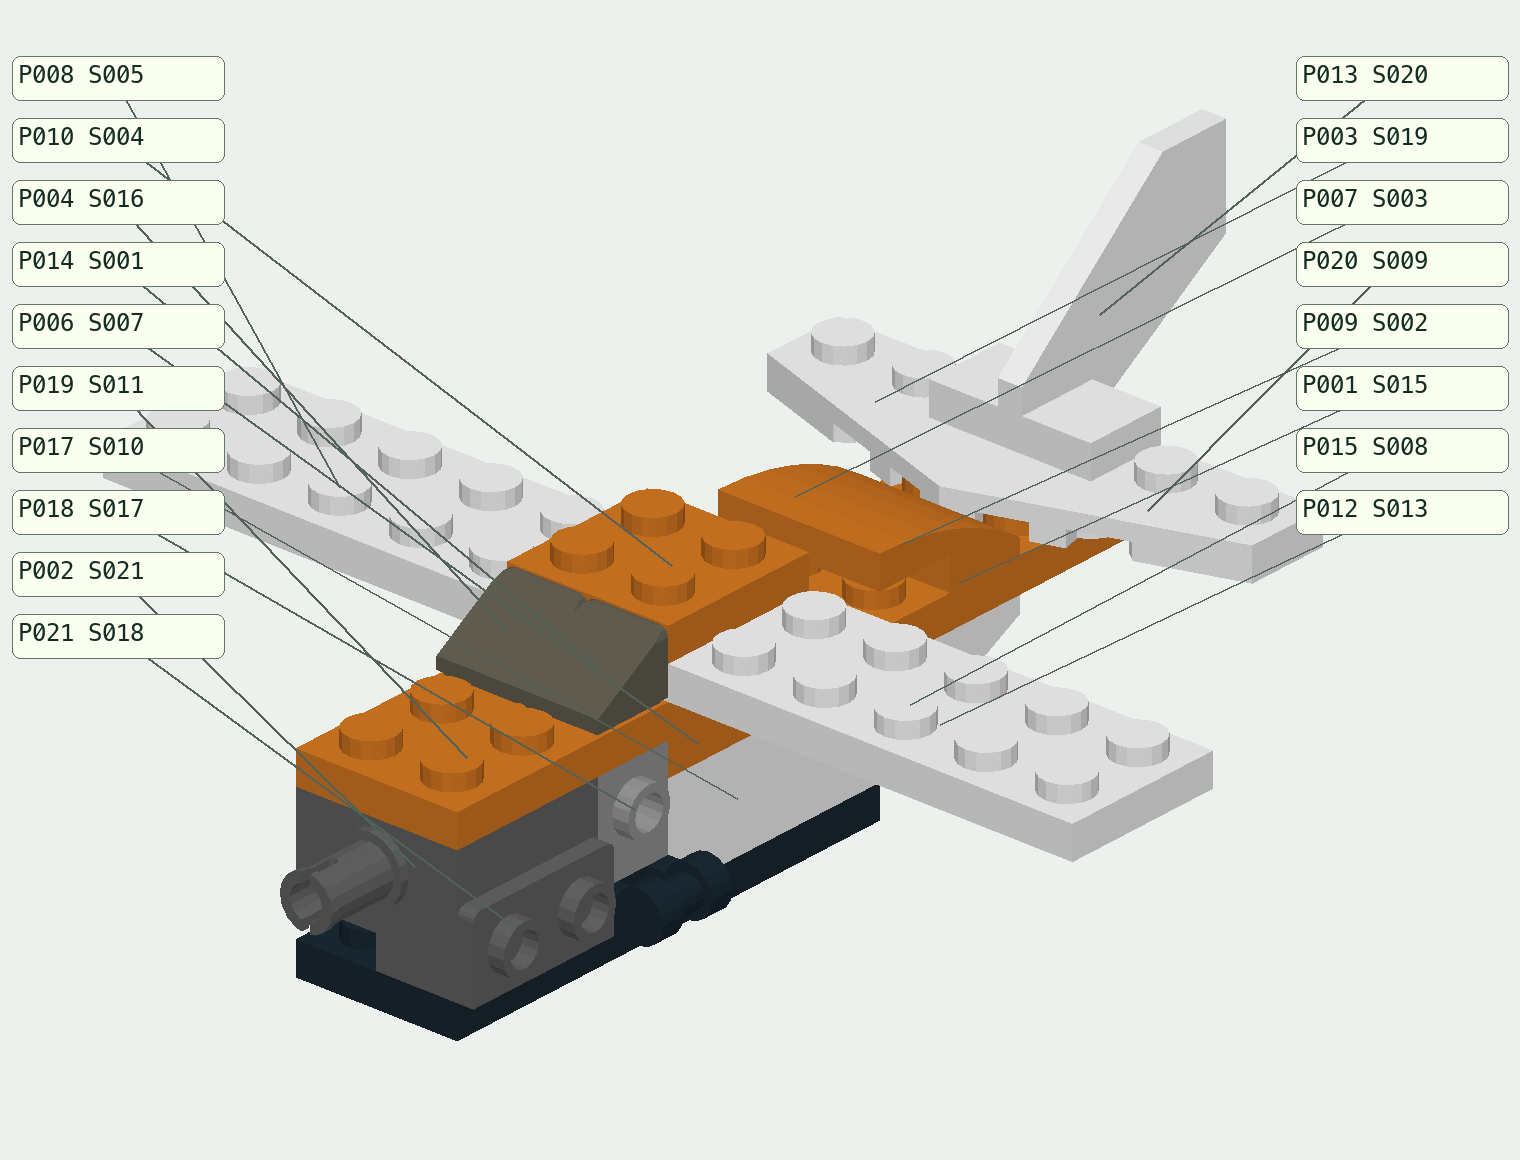
\includegraphics[width=\linewidth]{figures/reconfigure-34.png}\\
\small (d) Exact partial target, action 34.
\end{minipage}
\caption{Authoritative airframe reconfiguration replay, identity seed 31,
rendered from original LDraw triangles with source poses unchanged.
Eight initially mismatched sites require 34 successful actions and at least
15 detachments under the certified fixed paths. All displayed states remain
connected to the clamped base. Despite this cost, the privileged static
relation rule solves the task; length and rework do not certify deep search.
Frame hashes and exact occupancy are evaluator-side provenance artifacts.}
\end{figure*}

\section{Limitations and unresolved review concerns}
This release repairs measurement and one demonstrated probe shortcut; it
does not resolve the small number of source families, establish support
rerouting, or show empirical model shortsightedness.
Relations can be recovered or memorized in a public small bank, so held-out
source acquisition and external replication remain necessary.
No visual-perception or human study has been conducted.
Explicit image tracks make such studies possible but do not provide their
results. Image catalogs and fixed sites also simplify correspondence.

The physical abstraction excludes alternative insertion paths, rotation,
simultaneous subassembly moves, gravitational dynamics, clutch forces,
hand access and actual construction. Renderer fidelity is not a validation
of these omitted phenomena. There is no claim of general D2--D4 difficulty,
maximum planning horizon, CVPR readiness, or immunity to unknown shortcuts.
A strong next release needs new independently qualified mechanisms that
challenge the static relation baseline, more source groups, and preregistered
image-versus-structured model and human experiments.

\begin{thebibliography}{9}\small
\bibitem{ltron} LTRON / Break and Make. arXiv:2207.13738.
\url{https://arxiv.org/abs/2207.13738}.
\bibitem{instructionet} InstructioNet. arXiv:2410.01111.
\url{https://arxiv.org/abs/2410.01111}.
\bibitem{legopuzzles} LEGO-Puzzles. arXiv:2503.19990.
\url{https://arxiv.org/abs/2503.19990}.
\bibitem{phyblock} PhyBlock. arXiv:2506.08708.
\url{https://arxiv.org/abs/2506.08708}.
\bibitem{composer} Brick-Composer. arXiv:2606.05445.
\url{https://arxiv.org/abs/2606.05445}.
\end{thebibliography}
\end{document}
